%% FEUP THESIS STYLE for LaTeX2e
%% how to use feupteses (portuguese version)
%%
%% FEUP, JCL & JCF, 31 Jul 2012
%%
%% PLEASE send improvements to jlopes at fe.up.pt and to jcf at fe.up.pt
%%
%% Example for PDI course
%%

%%========================================
%% Commands: pdflatex tese
%%           bibtex tese
%%           makeindex tese (only if creating an index) 
%%           pdflatex tese
%% Alternative:
%%          latexmk -pdf tese.tex
%%========================================

\documentclass[11pt,a4paper,twoside,openright]{report}

%% For iso-8859-1 (latin1), comment next line and uncomment the second line
\usepackage[utf8]{inputenc}
%\usepackage[latin1]{inputenc}

%% Portuguese version

%% MIEEC options
%\usepackage[portugues,mieec]{feupteses}
%\usepackage[portugues,mieec,juri]{feupteses}
%\usepackage[portugues,mieec,final]{feupteses}
%\usepackage[portugues,mieec,final,onpaper]{feupteses}

%% For other degrees
\usepackage[portugues]{feupteses} % you must define the degree bellow

%% Options: 
%% - portugues: titles, etc in portuguese
%% - onpaper: links are not shown (for paper versions)
%% - backrefs: include back references from bibliography to citation place

%% Uncomment to create an index (at the end of the document)
%\makeindex

%% Path to the figures directory
%% TIP: use folder ``figures'' to keep all your figures
\graphicspath{{figures/}}

%%----------------------------------------
%% TIP: if you want to define more macros, use an external file to keep them
%some macro definitions

% format
\newcommand{\class}[1]{{\normalfont\slshape #1\/}}

% entities
\newcommand{\Feup}{Faculdade de Engenharia da Universidade do Porto}

\newcommand{\ecat}{\emph{EtherCAT}}
\newcommand{\arduino}{\emph{Arduino UNO}}
\newcommand{\raspi}{\emph{Raspberry Pi}}

%%----------------------------------------

%%========================================
%% Start of document
%%========================================
\begin{document}

%%----------------------------------------
%% Information about the work
%%----------------------------------------
\title{Ethernet de tempo real para aplicações robóticas}
\author{Simão Paulo Marques de Amorim}

\degree{\textsc{Preparação da dissertação}}
%% Uncomment next line for date of submission
%\thesisdate{31 de Julho de 2008}

%% Comment next line for copyright text if not used
\copyrightnotice{Simão Amorim, 2020}

\supervisor{Orientador}{Paulo José Lopes Machado Portugal}

%% Uncomment next line if necessary
%\supervisor{Co-orientador}{Nome de Outro Orientador}

%% Uncomment committee stuff in the final version if used
%\committeetext{Aprovado em provas públicas pelo Júri:}
%\committeemember{Presidente}{Nome do presidente do júri}
%\committeemember{Arguente}{Nome do arguente do júri}
%\committeemember{Vogal}{Nome do vogal do júri}
%\signature

%% Specify cover logo (in folder ``figures'')
\logo{uporto-feup.pdf}
 
%% Uncomment next line for additional text  below the author's name (front page)
% \additionalfronttext{Preparação da Dissertação}

%%----------------------------------------
%% Preliminary materials
%%----------------------------------------

% remove unnecessary \include{} commands
\begin{Prolog}
  \chapter*{Abstract}
%\addcontentsline{toc}{chapter}{Abstract}
We live in an increasingly digital and computerised world where there is a constant need for interconnection between everything and everyone.
Ethernet networks quickly became the communication standard in office and home environments, but their adoption in the industrial environment has been much slower.
This reduced speed of adoption is mainly due to the non-deterministic communication that Ethernet network provides, which does not make it a viable option for automation and robotics systems that require predictable and deterministic communications.
Modern automation and robotic systems do not escape the accelerated need for constant interconnection and, therefore, it is necessary to adapt them, taking into account their real-time requirements.
There are several well-established real-time Ethernet network solutions on the market, but we find the same gap on all of them: the scarcity of educational and demonstration equipment.

This document aims at presenting a solution for this gap, describing a distributed control system developed with education in mind.
The presented system focuses on the variable that mostly contributes to the deterministic characteristic of real-time Ethernet networks: the network cycle time.
The main objective is to develop a conceptual distributed control system capable of producing experimental data that demonstrates the impact that the communication network's cycle time has on control applications.
The proposed system will base itself on the implementation of a slave device for the EtherCAT network, implemented on a Raspberry Pi platform, and on the description of a possible implementation of a master device for the same network.
The implementation of the master device will purposely not be specified in detail to encourage greater involvement from the users of this system in implementing their own educational or demonstration system.

The document will begin with a presentation of the context in which this work was developed, followed by the motivation that led to the beginning of the project and a presentation of the objectives that we propose to achieve.
The state-of-the-art will consist of a presentation of real-time Ethernet networks in a generic way and an in-depth presentation of the working principle and characteristics of the EtherCAT network.
The presentation of generic real-time Ethernet networks will describe the existing categories and different approaches to the problem of non-deterministic communication in Ethernet networks.
The presentation and description of the architecture of the proposed distributed control system will follow.
Next, an explanation on how the implementation of the slave device was planned and executed, both in terms of hardware and software.
Finally, experimental results will also be presented.
These prove that the developed concept is valid and fulfils the intended characteristics.


\chapter*{Resumo}
%\addcontentsline{toc}{chapter}{Resumo}
Vivemos num mundo cada vez mais digital e informatizado onde existe uma constante necessidade de interligação entre tudo e todos.
As redes Ethernet rápidamente se tornaram no stardard da comunicação em ambientes empresariais e domésticos, mas a sua adoção no ambiente industrial tem sido bastante mais lenta.
Esta reduzida velocidade de adoção deve-se principalmente à comunicação não-determinística que a rede Ethernet proporciona, o que não a torna uma opção viável para sistemas de automação e robótica que necessitão de comunicações previsíveis e determinísticas.
Os automatismos e sistemas robóticos modernos não escapam à acelerada necessidade de constante interligação e, por isso, é necessário adaptá-los tendo em consideração os seu requisitos de tempo-real.
Existem no mercado várias soluções de redes Ethernet de comunicação de tempo real, já bem estabelecidas, mas em todas se encontra a mesma lacuna: a escassez de equipamento educativo e de demostração das mesmas.

O presente documento pretende apresentar uma solução para tal lacuna, descrevendo um sistema baseado em controlo distribuido desenvolvido a pensar na educação.
O sistema apresentado foca-se na variável com maior impacto na característica determinística das redes de Ethernet de tempo-real: o tempo de ciclo da rede.
O objectivo principal é desenvolver um conceito de um sistema de controlo distribuído capaz de produzir dados experimentais que demonstrem o impacto que o tempo de ciclo da rede de comunicação tem em aplicações de controlo.
O sistema proposto será baseado na implementação de um dispositivo escravo para a rede EtherCAT, implementado numa plataforma Raspberry Pi e na descrição de uma possível implementação de um dispositivo mestre para a mesma rede.
A implementação do dispositivo mestre será propositadamente deixada em aberto para incitar um maior envolvimento dos utilizadores deste sistema na implementação do seu próprio sistema educacional ou de demonstração.

O documento iniciará com uma apresentação do contexto em que este trabalho foi desenvolvido, seguido da motivação que levou à realização do projeto e da apresentação dos objetivos que propomos cumprir.
A revisão bibliográfica consistirá na apresentação de redes Ethernet de tempo-real de uma forma genérica e na apresentação aprofundada do modo de funcionamento e características da rede EtherCAT.
A apresentação de redes Ethernet de tempo-real genérica irá descrever as várias categorias existentes e as diferentes abordagens ao problema da falta de determinismo na comunicação Ethernet.
Seguir-se-á a apresentaçao e descrição da arquitetura do sistema de controlo distribuído proposto.
Seguidamente será explicado como foi planeada e executada a implementação do dispositivo escravo, tanto em termos de hardware como software.
Finalmente também irão ser apresentados resultados experimentais que provam que o conceito desenvolvido é válido e cumpre com as características pretendidas.

 % the abstract
%   \chapter*{Acknowledgements}
%\addcontentsline{toc}{chapter}{Agradecimentos}
I want to thank professor Paulo Portugal for his continuous availability  to provide me with the best and most informed feedback possible, during all stages of the project.
Even though getting feedback has not always been easy due to the full-remote work conditions that the CODIV-19 pandemic imposed, professor Paulo Portugal made sure that all interactions were used to the fullest of what was possible, every single time.

\bigskip
I would also like to thank my family for putting up with my working habits and routines while we were all working from home.
Sometimes it wasn't easy to reconcile work and personal life, but these were definitely times where everyone had to adapt to a new reality.
As such, I'm thankful for being able to  have my own time management and working habits, but I'm also thankful that my family advised me from overworking at certain times.

\bigskip
I want to dedicate this work to my good friend Ania who helped me get through some rough times on my personal life.
Sometimes life throws a curve ball at us and suddenly nothing seems to be going the right way.
But, eventually, things become easier to overcome, especially when one has a friend that motivates us and pushes us to do our best, no matter the circumstances.

\vspace{10mm}
\flushleft{Sim\~{a}o Amorim}
  % the acknowledgments
%   \cleardoublepage
\thispagestyle{plain}

\vspace*{8cm}

\begin{flushright}
%   \textsl{``You should be glad that bridge fell down. \\
%           I was planning to build thirteen more to that same design''} \\
%\vspace*{1.5cm}
%           Isambard Kingdom Brunel
	\textsl{``Tell me and I forget. Teach me and I remember. Involve me and I learn.''}\\
	\vspace*{1.5cm}
	Benjamin Franklin
\end{flushright}
    % initial quotation if desired
  \cleardoublepage
  \pdfbookmark[0]{Conteúdo}{contents}
  \tableofcontents
%   \cleardoublepage
%   \pdfbookmark[0]{Lista de Figuras}{figures}
%   \listoffigures
%   \cleardoublepage
%   \pdfbookmark[0]{Lista de Tabelas}{tables}
%   \listoftables
  \chapter*{Abreviaturas e Símbolos}
%\addcontentsline{toc}{chapter}{Abbreviations}
\chaptermark{ABREVIATURAS E SÍMBOLOS}

\begin{flushleft}
\begin{tabular}{l p{0.8\linewidth}}
ADT      & Abstract Data Type\\
ANDF     & Architecture-Neutral Distribution Format\\
API      & Application Programming Interface\\
CAD      & Computer-Aided Design\\
CASE     & Computer-Aided Software Engineering\\
CORBA    & Common Object Request Broker Architecture\\
UNCOL    & UNiversal COmpiler-oriented Language\\
Loren    & Lorem ipsum dolor sit amet, consectetuer adipiscing
elit. Sed vehicula lorem commodo dui\\
WWW      & \emph{World Wide Web}
\end{tabular}
\end{flushleft}

  % the list of abbreviations used
\end{Prolog}

%%----------------------------------------
%% Body
%%----------------------------------------

\StartBody

%% TIP: use a separate file for each chapter
\chapter{Introdução} \label{chap:intro}




\section{Contexto}\label{sec:contexto}

A recente digitalização da indústria introduz exigências cada vez maiores
de comunicações robustas, fiáveis e determinísticas na área da automação
industrial, em especial nas aplicações com requisitos de tempo-real.
Nos últimos anos tem-se assistido a uma crescente utilização de redes
industriais baseadas na tecnologia \textit{Ethernet}. Geralmente
denominadas redes de \textit{Ethernet} Industrial e de Tempo-Real, estas
tecnologias são adaptações da tecnologia \textit{Ethernet} original (IEEE
802.3) com o objetivo de interligar os dispositivos de um sistema com
requisitos de temporais exigentes. As soluções \textit{EthernetIP},
\textit{Profinet} e \ecat são os exemplos mais comuns deste tipo de redes
de comunicação.

A área da robótica industrial é um ótimo exemplo de que a utilização de
redes \textit{Ethernet} de tempo-real faz sentido. A sincronização de
ações entre componentes e a entrega e/ou difusão de mensagens cumprindo
intervalos de tempo determinísticos são apenas duas caraterísticas que
tornam a utilização destas redes quase indispensável em sistemas robóticos
modernos.


\section{Motivação}\label{sec:motivacao}

A forte presença das redes \textit{Ethernet} de tempo-real na industria
introduz a necessidade de dar formação acerca deste tema aos novos
técnicos e engenheiros da área. É, portanto, necessário colmatar a falta
de formação acerca deste tema na oferta formativa do curso de Engenharia
Eletrotécnica e de Computadores da FEUP\footnote{Faculdade de Engenharia
da Universidade do Porto}. A escassez no mercado de material didático de
formação restringe o tipo de formação possível a bases puramente teóricas.
Assim pretende-se desenvolver um sistema de demonstração intuitivo capaz
de evidênciar as capacidades e limitações destas redes, que será
posteriormente incluído nas atividades letivas do curso.

Atendendo à atual disponibilidade de material de redes \ecat presente na
FEUP, decidiu-se utilizar esta tecnologia para o desenvolvimento do
demonstrador em questão.


\section{Objetivos}\label{sec:objetivos}

O objetivo fundamental desta dissertação é o efetivo desenvolvimento de
uma plataforma robótica de demonstração prática e intuitiva da rede \ecat
e da sua respetiva aplicação de controlo. Para isto, um estudo aprofundado
da tecnologia e das funcionalidades deste protocolo é fundamental para
que o sistema final possa apresentar um leque alargado das suas
capacidades e limitações.

Como o foco da demonstração é a utilização destas tecnologias em
aplicações robóticas, a plataforma deverá ser baseada no controlo de
trajetórias de eixos, com uma configuração que permita, entre outros
aspetos, demonstrar as caraterísticas da rede \ecat ao nível da
sincronização temporal (sincronização de ações) e da resposta temporal
(tráfego em tempo-real) da aplicação de controlo.
 
\chapter{Revisão Bibliográfica} \label{chap:sota}


\section{Definição e caraterização do problema}\label{sec:problem}

Com a modernização constante da indústria e consequente crescente exigência
de conetividade de todo o tipo de equipamentos, é imperativa a introdução
de novas soluções tecnológicas que satisfaçam estes requisitos modernos
mas que também mantenham a compatibilidade com as exigências satisfeitas
pelos sistemas atualmente em uso.

Quando nos referimos à área da robótica, exigências temporais como o
período, a latência e a periodicidade da malha de controlo são fulcrais
para o funcionamento estável do sistema. Ora, a crescente exigência de
conetividade moderna instiga à utilização de redes de comunicação no
ambiente industrial. Quando o controlo de diversas áreas num equipamento
é feito de modo central num PLC ou micro-controlador, a sincronização de
alteração de estados de saídas é trivial, pois basta garantir que ambas
são atualizadas no mesmo ciclo de processamento. Quando se pretende
introduzir uma rede de comunicação entre o processamento central e o
controlo das saídas e/ou a aquisição das entradas, é crucial garantir
que não existem atrasos significativos na transmissão da informação
na rede e garantir a sincronização entre as atualizações das saídas
nos diversos escravos.

Nos últimos anos, várias implementações e estudos já foram realizados
com manipuladores robóticos utilizando redes de comunicação na malha de
controlo como \cite{Zhang18}, \cite{leiwang2010} ou muito recentemente
\cite{deremetz2020}. No entanto, todas elas se focam na vertente mais
industrial e técnica da solução e praticamente não existem implementações
focadas no ensino.

% económico
Um demonstrador focado no ensino deve ter caraterísticas apelativas de
modo a que a sua utilização possa ser o mais generalizada possível. O
primeiro objetivo deverá ser o desenvolvimento de um produto económico
de modo a que este possa ser adquirido em larga escala pelos
estabelecimentos de ensino. É também preciso considerar que no ambiente
de ensino, é mais provável acontecerem situações de utilização indevida
de um equipamento do que em ambiente industrial, onde geralmente apenas
pessoas qualificadas estão autorizadas a interagir com o mesmo, e portanto
uma possível avaria do produto não pode trazer prejuízos avultados à
instituição e/ou ao estudante. Naturalmente, esta redução no custo
implicará sempre uma redução na qualidade do produto final face a um
desenvolvimento de nível industrial, mas essa não é uma caraterística
fundamental de um demonstrador didático.

% implementação simples
Muitas vezes o momento em que nos é apresentada uma tecnologia desconhecida
através de um demostrador didático surgem questões acerca do demostrador
propriamente dito e não na tecnologia que ele pretende demonstrar. Assim,
para minimizar este tipo de interferência na aprendizagem existem duas
possíveis soluções: utilizar uma ideia de base que seja tão simples que
não permita qualquer tipo de dúvida ou que o público alvo tenha um
conhecimento aprofundado da ideia de base. Considerando que o público alvo
deste demostrador são estudantes de mestrado na área da robótica,
o controlo de movimento e posição de um manipulador robótico são temas
bem conhecidos.

% componentes 'off the shelf'
Complementando a caraterística económica de um demonstrador educativo,
a utilização de componentes e sub-sistemas genéricos, denominados
componentes \emph{off-the-shelf}, facilita a aquisição dos mesmos tanto
para o fabrico como para reparações. Assim, é possível que o próprio
cliente faça uma reparação do produto, sendo que a ação mais simples será
a troca do componente ou sub-sistema danificado.

% modularidade
A utilização de componentes e sub-sistemas genéricos leva-nos a um ponto
importante de demonstradores educativos: a modularidade. Um sistema
dividido em sub-sistemas mais simples que se focam numa única tarefa é um
sistema modular. Cada sub-sistema por si é simples, fácil de implementar,
interpretar e diagnosticar. A conjugação dos diferentes sub-sistemas,
encadeados e inter-ligados permite obter um sistema mais complexo com a
vantagem de que o seu desenvolvimento e eventual diagnóstico possa ser
feito por partes, o que simplifica tal processo, proporcionando também a
possibilidade de este ser paralelizado. Esta modularidade permite que,
no contexto de aprendizagem, seja mais fácil e rápido interpretar o
funcionamento de cada sub-sistema e, consequentemente, interpretar o
funcionamento geral do sistema.

% intuitivo
Por fim, a caraterística mais importante de qualquer demonstrador
educativo, e razão pela qual estes existem, é o seu caráter intuitivo.
Qualquer utilizador tem de ser capaz de, através do próprio funcionamento
do demonstrador, entender o conceito base em exposição. Em ambiente
educacional é muito importante fornecer este tipo de contacto com a
tecnologia para que os estudantes possam sedimentar os conhecimentos com
mais facilidade e de uma forma mais duradoura. % TODO arranjar citação para isto


\section{\ecat}\label{sec:ethercat}

A rede \ecat\ é uma rede de \emph{Ethernet} industrial que usa a
especificação padrão IEEE 802.3 \cite[]{ieee:IEEEStandardEthernet} para
definir o formato dos \emph{frames} e camada física a utilizar, mas
introduz uma maneira diferente de os processar.

Esta nova forma de processamento permite uma comunicação com todos os
dispositivos presentes na rede com apenas um \emph{frame}. \ecat\ utiliza
uma tipologia de comunicação \emph{Master/Slave}, tipicamente implementada
numa arquitetura de rede encadeada (\emph{daisy-chain}), mas permite várias
outras arquiteturas.
% TODO: Citar aqui algo que explicite as varias arquiteturas

\subsection{Arquiteture de rede encadeada (\emph{daisy-chain})}
\label{sec:daisychain}
Apenas o dispositivo mestre pode iniciar um \emph{frame} de comunicação
e os dispositivos escravos limitam-se a ler a parte informação contida
no \emph{frame} que lhes é endereçada. Ao mesmo tempo, cada dispositivo
escravo pode introduzir informação sua  no \emph{frame} antes de o enviar
para o dispositivo seguinte.

\subsection{sincronização de relógios}
% TODO

\subsection{Conclusão}
Estas caraterísticas permitem que o dispositivo mestre seja implementado
em qualquer tipo de dispositivo que contenha uma porta de comunicação 
\emph{Ethernet}. Os dispositivos escravo utilizam um \emph{EtherCAT Slave
Controller} (ESC) que processa os \emph{frames} fazendo com que a velocidade
e tempos de resposta da rede sejam previsíveis e independentes dos 
dispositivos escravo que existam na rede. Assim, é possível a utilização
de dispositivos escravo implementados em arquiteturas de computação
diferentes dentro da mesma rede \ecat.


\section{Soluções propostas} \label{sec:solution}

Para atingir os objetivos propostos por esta dissertação, foram propostas 
duas possíveis soluções. Ambas são apresentadas de seguida sendo que
maior ênfase será dada na última, pois é a proposta que se mostra mais
adequada ao estudo em questão.

Ambas as soluções têm por base o controlo de movimento através da velocidade
e/ou posição de um sistema robótico de múltiplos eixos. Fazendo uso de
uma arquitetura de controlo distribuída interligada por uma rede \ecat\
em tipologia encadeada (secção \ref{sec:daisychain}). Esta arquitetura
será constituída por um dispositivo mestre implementado num micro-computador
\raspi\, programado através das linguagens descritas no padrão
IEC 61161-3. Os dispositivos escravo, que farão a interface com os atuadores,
sensores e interface de comando, serão implementados através de placas
\arduino\ agrupado com o adaptador \emph{EasyCAT} da \cite{ABT:EasyCAT}.
Um esquema da arquitetura pretendida é mostrado na figura
\ref{fig:network-architecture}.

\begin{figure}
 \centering
 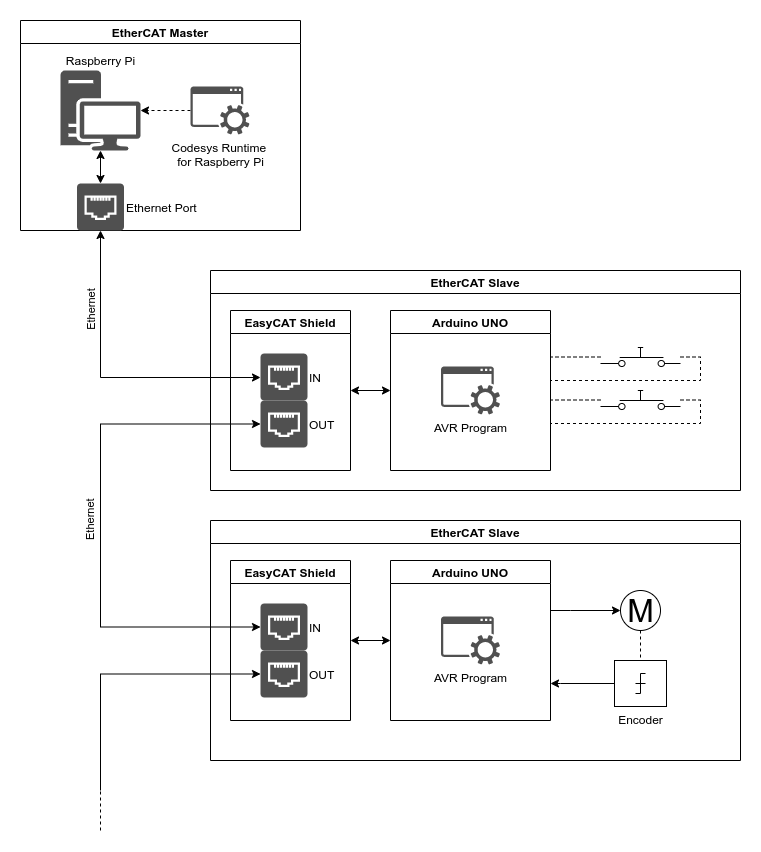
\includegraphics[width=\linewidth]{network-diagram_transparent.png}
 \caption{Arquitetura da rede \ecat\ pretendida}
 \label{fig:network-architecture}
\end{figure}



\subsection{Controlo de discos perfurados}\label{sec:discs_project}

%\subsubsection{O conceito}
A primeira solução idealizada no contexto desta dissertação baseia-se num
sistema de controlo e sincronização de discos rotativos independentes.
Estes são perfurados na extremidade de maneira a que possam ser momentaneamente atravessados por um feixe de laser. Este último será fixo numa das extremidades
do demonstrador com orientação que permita atravessar todos os discos presentes
no sistema, ficando visível na extremidade oposta do demonstrador. Assim,
com estes discos acoplados a motores DC com codificadores de posição (\emph{encoder}),
controlados de forma independente por placas \arduino\ a funcionar em modo
de \ecat\ \emph{slave}, é possível criar diferentes cenários de controlo
cujo objetivo seja periodicamente alinhar as furações dos discos com o
feixe laser, permitindo que este seja viaje até à extremidade oposta.

Para complementar este conceito, será necessário permitir que o estado
do ponteiro laser (ligado ou desligado) seja controlado pelo sistema,
criando uma camada adicional de complexidade que ajuda a entender a
importância da sincronização de relógios nas redes de comunicação de
tempo real. Desta forma é possível ativar o ponteiro laser apenas quando
o sistema  determinar que os discos estão na orientação correta, fazendo
com seja mais percetível a importância da sincronização de relógios para
que seja possível uma atualização síncrona do estado das saídas.

%\subsubsection{Flexibilidade}
Idealmente esta soluçao deverá permitir efetuar o mesmo controlo mas não
usando as capacidades da rede \ecat\ e usando apenas comunicação
\emph{Ethernet} simples, o que permitirá efetuar uma comparação efetiva
destes protocolos e demonstrar que em ambientes de rede de comunicação
tradicionais não existem considerações de tempo real nem de sincronização.
Esta funcionalidade implicará verificar se os adaptadores \emph{EasyCAT}
permitem comunicação \emph{Ethernet} simples ou até de outros protocolos
de \emph{Ethernet} industrial (p.ex. \emph{Modbus TCP}), mas até ao momento
ainda não o foi possível determinar.

%\subsubsection{Conclusão}
Desta forma evidenciam-se as capacidades da rede \ecat\ no que diz
respeito à resposta temporal, sincronização de relógios e capacidade de
transferência de dados num sistema cujo conceito é acessível a qualquer
estudante de engenharia eletrotécnica.


\subsection{Seguimento de um traçado com um braço robótico}



% \chapter{Plano de trabalho}\label{chap:chap3}

Neste capítulo apresenta-se o planeamento de tarefas, seus objetivos,
faseamento e metodologia de abordagem. No final será feita uma breve
apresentação das tecnologias e ferramentas escolhidas que permitirão
realizar as tarefas e cumprir os objetivos propostos.


\section{Tarefas, objetivos e metodologia de abordagem}

Para poder iniciar os trabalhos com uma rede \ecat\, será necessário,
naturalmente, ter uma rede provisória funcional onde se possa iniciar o
desenvolvimento do software de controlo. Para isto, está planeada a
montagem de uma pequena rede \ecat\ através de um \raspi\ como dispositivo
mestre e, no mínimo, dois conjuntos \arduino\ + \emph{EasyCAT} como
dispositivos escravo, cada um com um motor associado.


\subsection{Calendarização}
% TODO

Loren ipsum dolor sit amet, consectetuer adipiscing elit. 
Praesent sit amet sem. Maecenas eleifend facilisis leo. Vestibulum et
mi. Aliquam posuere, ante non tristique consectetuer, dui elit
scelerisque augue, eu vehicula nibh nisi ac est. Suspendisse elementum
sodales felis. Nullam laoreet fermentum urna. 

Duis eget diam. In est justo, tristique in, lacinia vel, feugiat eget,
quam. Pellentesque habitant morbi tristique senectus et netus et
malesuada fames ac turpis egestas. Fusce feugiat, elit ac placerat
fermentum, augue nisl ultricies eros, id fringilla enim sapien eu
felis. Vestibulum ante ipsum primis in faucibus orci luctus et
ultrices posuere cubilia Curae; Sed dolor mi, porttitor quis,
condimentum sed, luctus in. 


\subsection{Tecnologias e ferramentas a usar}
% TODO
Loren ipsum dolor sit amet, consectetuer adipiscing elit. 
Praesent sit amet sem. Maecenas eleifend facilisis leo. Vestibulum et
mi. Aliquam posuere, ante non tristique consectetuer, dui elit
scelerisque augue, eu vehicula nibh nisi ac est. Suspendisse elementum
sodales felis. Nullam laoreet fermentum urna. 

Duis eget diam. In est justo, tristique in, lacinia vel, feugiat eget,
quam. Pellentesque habitant morbi tristique senectus et netus et
malesuada fames ac turpis egestas. Fusce feugiat, elit ac placerat
fermentum, augue nisl ultricies eros, id fringilla enim sapien eu
felis. Vestibulum ante ipsum primis in faucibus orci luctus et
ultrices posuere cubilia Curae; Sed dolor mi, porttitor quis,
condimentum sed, luctus in. 

% \chapter{Mais um Capítulo}\label{chap:chap4}

Neste capítulo mostra-se apenas o formato da dissertação.

Ipsum dolor sit amet, consectetuer
adipiscing elit.  Praesent sit amet sem. 
Maecenas eleifend facilisis leo. Vestibulum et
mi. Aliquam posuere, ante non tristique consectetuer, dui elit
scelerisque augue, eu vehicula nibh nisi ac est. 
Suspendisse elementum sodales felis. 
Nullam laoreet fermentum urna. 

\section{Secção Exemplo}

Lorem ipsum dolor sit amet, consectetuer adipiscing elit. Integer
hendrerit commodo ante. Pellentesque nibh libero, aliquam at, faucibus
id, commodo a, velit. Duis eleifend sem eget leo. Morbi in
est. Suspendisse magna sem, varius nec, hendrerit non, tincidunt quis,
quam. Aenean congue. Vivamus vel est sit amet sem iaculis
posuere. Cras mollis, enim vel gravida aliquam, libero nunc
ullamcorper dui, ullamcorper sodales lectus nulla sed urna. Morbi
aliquet porta risus. Proin vestibulum ligula a purus. Maecenas a
nulla. Maecenas mattis est vitae neque auctor tempus. Etiam nulla dui,
mattis vitae, porttitor sed, aliquet ut, enim. Cras nisl magna,
aliquet et, laoreet at, gravida ac, neque. Sed id est. Nulla dapibus
dolor quis ipsum rhoncus cursus. 

Etiam nisi est, dignissim sodales, fermentum id, pulvinar ac,
eros. Duis id orci. Nam pretium nisl ac augue. Ut adipiscing magna
eget est. Curabitur varius. Nulla facilisi. Pellentesque sit amet
neque ac dui accumsan blandit. Donec mauris felis, egestas sit amet,
convallis ac, dignissim quis, dolor. Maecenas cursus tortor vel
leo. Quisque tristique. Nunc augue odio, tincidunt in, dapibus sed,
ultricies sit amet, lorem. In hac habitasse platea dictumst. Praesent
iaculis, lacus hendrerit tempor sodales, libero tellus aliquet orci,
ut rhoncus massa lectus quis erat. Pellentesque quis dolor nec tortor
rhoncus convallis. Aliquam erat volutpat. Fusce placerat, magna eu
imperdiet lobortis, augue massa blandit turpis, a consectetuer quam
arcu sit amet risus. Suspendisse potenti. Praesent sapien metus,
interdum vitae, fermentum id, faucibus ut, lorem. Nunc iaculis purus
id tortor. Aenean risus pede, laoreet ac, tristique sed, lobortis in,
turpis. 

Vestibulum et lorem in ligula viverra pharetra. Curabitur quis purus
in urna facilisis bibendum. Pellentesque at arcu accumsan velit
bibendum ornare. Praesent massa. Quisque dolor. In libero. Vestibulum
ac diam id leo feugiat blandit. Donec porta, tellus ac pellentesque
molestie, felis mauris viverra lacus, sed dignissim purus justo eu
justo. Proin iaculis, nunc eu volutpat volutpat, libero purus rutrum
enim, id euismod lacus lorem nec augue. Donec hendrerit lacinia
ante. Integer mollis vulputate orci. In pellentesque, metus pharetra
elementum pharetra, est purus bibendum turpis, eu pretium sapien
libero convallis odio. Cras sodales bibendum risus. Sed mattis nulla
non leo. Nulla nunc. Phasellus egestas sodales massa. Class aptent
taciti sociosqu ad litora torquent per conubia nostra, per inceptos
himenaeos. Pellentesque habitant morbi tristique senectus et netus et
malesuada fames ac turpis egestas. Etiam mi. 

\section{Mais uma Secção}

Lorem ipsum dolor sit amet, consectetuer adipiscing elit. Quisque
purus sapien, interdum ut, vestibulum a, accumsan ullamcorper,
erat. Mauris a magna ut leo porta imperdiet. Donec dui odio, porta in,
pretium non, semper quis, orci. Quisque erat diam, pharetra vel,
laoreet ac, hendrerit vel, enim. Donec tristique luctus risus. Fusce
dolor est, eleifend id, elementum sit amet, varius vitae, neque. Morbi
at augue. Ut sem ligula, auctor vitae, facilisis id, pharetra non,
lectus. Nulla lacus augue, aliquam eget, sollicitudin sed, hendrerit
eu, leo. Suspendisse ac tortor. Mauris at odio. Etiam vehicula. Nam
lacinia purus at nibh. Aliquam fringilla lorem ac justo. Ut nec
enim. Nunc ornare, eros eu facilisis tristique, nisl lorem lacinia
risus, non ullamcorper tellus urna et eros. Quisque eleifend tempus
metus. Nunc ipsum. 

Phasellus ullamcorper justo id risus. Nunc in leo. Mauris auctor
lectus vitae est lacinia egestas. Nulla faucibus erat sit amet lectus
varius semper. Praesent ultrices vehicula orci. Nam at metus. Aenean
eget lorem nec purus feugiat molestie. Phasellus fringilla nulla ac
risus. Aliquam elementum aliquam velit. Aenean nunc odio, lobortis id,
dictum et, rutrum ac, ipsum. Aenean tellus magna, lacinia eget,
bibendum ut, interdum sit amet, ipsum. Class aptent taciti sociosqu ad
litora torquent per conubia nostra, per inceptos himenaeos. Mauris
felis lacus, dapibus sit amet, pretium feugiat, aliquet non,
purus. Aliquam elementum, diam quis porttitor gravida, sem sapien
iaculis nulla, ut pharetra odio felis a metus. Nulla lacus ipsum,
tristique ut, dapibus sed, mollis et, justo. Vivamus non ipsum sed
ligula placerat ultrices. Maecenas dictum leo adipiscing
mauris. Vestibulum tristique, lacus a consequat suscipit, nunc dui
sollicitudin arcu, non interdum libero est eget tortor. Ut eget neque
quis leo tempor dictum. 

Quisque ullamcorper. Aliquam vel magna. Sed pulvinar dictum
ligula. Sed ultrices dolor ut turpis. Vivamus sagittis orci malesuada
arcu venenatis auctor. Proin vehicula pharetra urna. Aliquam egestas
nunc quis nisl. Donec ullamcorper. Nulla purus. Ut suscipit lacus
vitae dui. Mauris semper. Ut eget sem. Integer orci. Nam vitae dui
eget nisi placerat convallis. 

Sed id lorem. Proin gravida bibendum lacus. Sed molestie, urna quis
euismod laoreet, diam dolor dictum diam, vitae consectetuer leo ipsum
id ante. Integer eu lectus non mauris pharetra viverra. In feugiat
libero ut massa. Morbi cursus, lorem sollicitudin blandit semper,
felis magna pellentesque lacus, ut rhoncus leo neque at tellus. Sed
mattis, diam eget eleifend tincidunt, ligula eros tincidunt diam,
vitae auctor turpis est vel nunc. In eu magna. Donec dolor metus,
egestas sit amet, ultrices in, faucibus sed, lectus. Etiam est enim,
vehicula pharetra, porta non, viverra vel, nunc. Ut non sem. Etiam nec
neque. Sed rhoncus, justo id imperdiet pharetra, mi tellus accumsan
neque, vitae volutpat tortor enim in odio. Nunc porta justo a
lorem. Nulla hendrerit odio vitae dolor. Suspendisse eu nisl.  

\section{Resumo ou Conclusões}

Proin vehicula pharetra urna. Aliquam egestas
nunc quis nisl. Donec ullamcorper. Nulla purus. Ut suscipit lacus
vitae dui. Mauris semper. Ut eget sem. Integer orci. Nam vitae dui
eget nisi placerat convallis. 

% \chapter{Conclusões e Trabalho Futuro} \label{chap:concl}

Proin sed justo eu sapien eleifend elementum. Pellentesque
habitant morbi tristique senectus et netus et malesuada fames ac
turpis egestas. Vivamus quam lacus, pharetra vel, aliquam vel,
volutpat sed, nisl. 

\section{Satisfação dos Objectivos}

Lorem ipsum dolor sit amet, consectetuer adipiscing elit. Etiam non
felis sed odio rutrum ultrices. Donec tempor dolor. Vivamus justo
neque, tempus id, ullamcorper in, pharetra non, tellus. Praesent eu
orci eu dolor congue gravida. Sed eu est. Donec pulvinar, lectus et
eleifend volutpat, diam sapien sollicitudin arcu, a sagittis libero
neque et dolor. Nam ligula. Cras tincidunt lectus quis nunc. Cras
tincidunt congue turpis. Nulla pede velit, sagittis a, faucibus vitae,
porttitor nec, ante. Nulla ut arcu. Cras eu augue at ipsum feugiat
hendrerit. Proin sed justo eu sapien eleifend elementum. Pellentesque
habitant morbi tristique senectus et netus et malesuada fames ac
turpis egestas. Vivamus quam lacus, pharetra vel, aliquam vel,
volutpat sed, nisl. 

Nullam erat est, vehicula id, tempor non, scelerisque at,
tellus. Pellentesque tincidunt, ante vehicula bibendum adipiscing,
lorem augue tempor felis, in dictum massa justo sed metus. Suspendisse
placerat, mi eget molestie sodales, tortor ante interdum dui, ac
sagittis est pede et lacus. Duis sapien. Nam ornare turpis et
magna. Etiam adipiscing adipiscing ipsum. Fusce sodales nisl a
arcu. Cras massa leo, vehicula facilisis, commodo a, molestie
faucibus, metus. Suspendisse potenti. Duis sagittis. Donec porta. Sed
urna. Maecenas eros. Vivamus erat ligula, pharetra sit amet, bibendum
et, fermentum sed, dolor. Nullam eleifend condimentum nibh. Integer
leo nibh, consequat eget, mollis et, sagittis ac, felis. Duis viverra
pede in pede. Phasellus molestie placerat leo. Praesent at tellus a
augue congue molestie. Proin sed justo eu sapien eleifend
elementum. Pellentesque habitant morbi tristique senectus et netus et
malesuada fames ac turpis egestas. 

\section{Trabalho Futuro}

Lorem ipsum dolor sit amet, consectetuer adipiscing elit. Aliquam
tempor tristique risus. Suspendisse potenti. Fusce id eros. In eu
enim. Praesent commodo leo. Nullam augue. Pellentesque tellus. Integer
pulvinar purus a dui convallis consectetuer. In adipiscing, orci vitae
lacinia semper, sapien elit posuere sem, ac euismod ipsum elit tempus
urna. Aliquam erat volutpat. Nullam suscipit augue sed
felis. Phasellus faucibus accumsan est. 

Aliquam felis justo, facilisis sit amet, bibendum ut, tempus ac,
dolor. Sed malesuada. Nunc non massa. In erat. Nulla
facilisi. Phasellus blandit, est in accumsan cursus, libero augue
elementum leo, vitae auctor mauris nisl ac tortor. Cras porttitor
ornare elit. Fusce at lorem. Sed lectus tortor, vestibulum id, varius
a, condimentum nec, lectus. Maecenas in nisi et magna pretium
aliquam. Pellentesque justo elit, feugiat nec, tincidunt a, dignissim
vel, ipsum. Sed nunc. Vestibulum ante ipsum primis in faucibus orci
luctus et ultrices posuere cubilia Curae; Aliquam tempus rhoncus
leo. Donec neque quam, cursus sit amet, ultricies varius, semper non,
pede. Donec porttitor. Sed aliquet feugiat elit.  

\vspace*{12mm}

Lorem ipsum dolor sit amet, consectetuer adipiscing elit. Phasellus
tellus pede, auctor ut, tincidunt a, consectetuer in, felis. Mauris
quis dolor et neque accumsan pellentesque. Donec dui magna,
scelerisque mattis, sagittis nec, porta quis, nulla. Vivamus quis
nisl. Etiam vitae nisl in diam vehicula viverra. Sed sollicitudin
scelerisque est. Nunc dapibus. Sed urna. Nulla gravida. Praesent
faucibus, risus ac lobortis dignissim, est tortor laoreet mauris,
dictum pellentesque nunc orci tincidunt tellus. Nullam pulvinar, leo
sed vestibulum euismod, ante ligula elementum pede, sit amet dapibus
lacus tortor ac nisl. Morbi libero. Integer sed dolor ac lectus
commodo iaculis. Donec ut odio.  
 

%% Comment next 2 commands if numbered appendices are not used
% \appendix
% \chapter{Loren Ipsum} \label{ap1:loren}

Depois das conclusões e antes das referências bibliográficas,
apresenta-se neste anexo numerado o texto usado para preencher a
dissertação.

\section{O que é o \emph{Loren Ipsum}?}

\emph{\textbf{Lorem Ipsum}} is simply dummy text of the printing and
typesetting industry. Lorem Ipsum has been the industry's standard
dummy text ever since the 1500s, when an unknown printer took a galley
of type and scrambled it to make a type specimen book. It has survived
not only five centuries, but also the leap into electronic
typesetting, remaining essentially unchanged. It was popularised in
the 1960s with the release of Letraset sheets containing Lorem Ipsum
passages, and more recently with desktop publishing software like
Aldus PageMaker including versions of Lorem Ipsum. 

\section{De onde Vem o Loren?}

Contrary to popular belief, Lorem Ipsum is not simply random text. It
has roots in a piece of classical Latin literature from 45 BC, making
it over 2000 years old. Richard McClintock, a Latin professor at
Hampden-Sydney College in Virginia, looked up one of the more obscure
Latin words, consectetur, from a Lorem Ipsum passage, and going
through the cites of the word in classical literature, discovered the
undoubtable source. Lorem Ipsum comes from sections 1.10.32 and
1.10.33 of ``de Finibus Bonorum et Malorum'' (The Extremes of Good and
Evil) by Cicero, written in 45 BC. This book is a treatise on the
theory of ethics, very popular during the Renaissance. The first line
of Lorem Ipsum, ``Lorem ipsum dolor sit amet\ldots'', comes from a line in
section 1.10.32.

The standard chunk of Lorem Ipsum used since the 1500s is reproduced
below for those interested. Sections 1.10.32 and 1.10.33 from ``de
Finibus Bonorum et Malorum'' by Cicero are also reproduced in their
exact original form, accompanied by English versions from the 1914
translation by H. Rackham.

\section{Porque se usa o Loren?}

It is a long established fact that a reader will be distracted by the
readable content of a page when looking at its layout. The point of
using Lorem Ipsum is that it has a more-or-less normal distribution of
letters, as opposed to using ``Content here, content here'', making it
look like readable English. Many desktop publishing packages and web
page editors now use Lorem Ipsum as their default model text, and a
search for ``lorem ipsum'' will uncover many web sites still in their
infancy. Various versions have evolved over the years, sometimes by
accident, sometimes on purpose (injected humour and the like). 

\section{Onde se Podem Encontrar Exemplos?}

There are many variations of passages of Lorem Ipsum available, but
the majority have suffered alteration in some form, by injected
humour, or randomised words which don't look even slightly
believable. If you are going to use a passage of Lorem Ipsum, you need
to be sure there isn't anything embarrassing hidden in the middle of
text. All the Lorem Ipsum generators on the Internet tend to repeat
predefined chunks as necessary, making this the first true generator
on the Internet. It uses a dictionary of over 200 Latin words,
combined with a handful of model sentence structures, to generate
Lorem Ipsum which looks reasonable. The generated Lorem Ipsum is
therefore always free from repetition, injected humour, or
non-characteristic words etc. 


%%----------------------------------------
%% Final materials
%%----------------------------------------

%% Bibliography
%% Comment the next command if BibTeX file not used, 
%% Assumes that bibliography is in ``myrefs.bib''
\PrintBib{myrefs}

%% Index
%% Uncomment next command if index is required, 
%% don't forget to run ``makeindex tese'' command
%\PrintIndex

\end{document}
